\begin{frame}{Beispiel: $H_{\mathrm{S}}$, $H_{\mathrm{SE}}$}
	\alt<1,2>{\begin{itemize}
		\item{Zeitentwicklung von S}
		\begin{itemize}
			\item{$U = \exp(-i \int\!\!\!H_{\mathrm{OS}}\dif t)$, spontane Entscheidung}
			\item{$U\ketneutrey = \frac{1}{\sqrt{2}}\del{\ketsmiley + \ketfrowny}$, $\rho_{\mathrm{S}} = \ketneutrey\braneutrey$}
		\end{itemize}
	\end{itemize}
				\begin{columns}
					 \alt<1>{\begin{column}{\textwidth}
					 	\vspace{0.25cm}
		 			 	\centering
		 			 	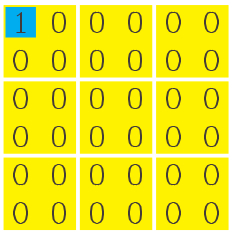
\includegraphics[scale=0.35]{graphics/subsystem_example_1_1.jpg}
					 	\end{column}}{}
					\alt<2>{\begin{column}{0.55\textwidth}
						\begin{beamerboxesrounded}{}
							\begin{align*}
							\rho^{\prime}_{\mathrm{S}} = U\rho_{\mathrm{S}}U^{\dagger}
							=&\frac{1}{2}(\ketsmiley\brasmiley + \ketsmiley\brafrowny \\ &+ \ketfrowny\brasmiley + \ketfrowny\brafrowny)
							\end{align*}
							\vspace{-0.5cm}
						\end{beamerboxesrounded}
					\end{column}
					\begin{column}{0.35\textwidth}
						 \centering
						 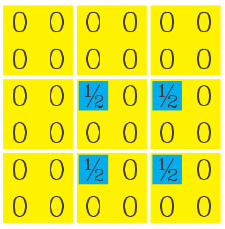
\includegraphics[scale=0.35]{graphics/subsystem_example_2_2.jpg}
					\end{column}}{}
				\end{columns}}{}	
	\alt<3>{\begin{itemize}
			\item{$H_{\mathrm{SE}}$: Dekohärenz des Subjekts}
		\end{itemize}
		\begin{columns}
			\begin{column}{0.55\textwidth}
				\begin{beamerboxesrounded}{}
					\begin{equation*}
					\rho^{\prime\prime}_{\mathrm{S}} = \frac{1}{2}(\ketsmiley\brasmiley + \ketfrowny\brafrowny)
					\end{equation*}
					\vspace{-0.5cm}
				\end{beamerboxesrounded}
			\end{column}
			\begin{column}{0.35\textwidth}
				\centering
				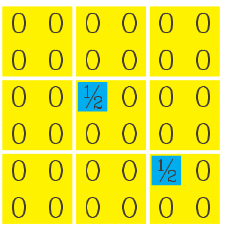
\includegraphics[scale=0.35]{graphics/subsystem_example_2_3.jpg}
			\end{column}
		\end{columns}
	\begin{itemize}
		\item{Auf welchen Zeitskalen läuft Dekohärenz im Gehirn ab?}
	\end{itemize}}{}			
		
\end{frame}